\section{Background and Motivation}
\label{sec:rmotivation}

RAMCloud~\cite{ramcloud} is a key-value store that keeps all data in
DRAM at all times and is designed to scale across thousands of commodity data
center servers. Each server can service millions of operations per
second, but its focus is on low access latency.  End-to-end read and durable
write operations take just 6~\us~and~15~\us,
respectively, on our hardware (\S\ref{sec:reval}).

\begin{figure}[t]
\centering
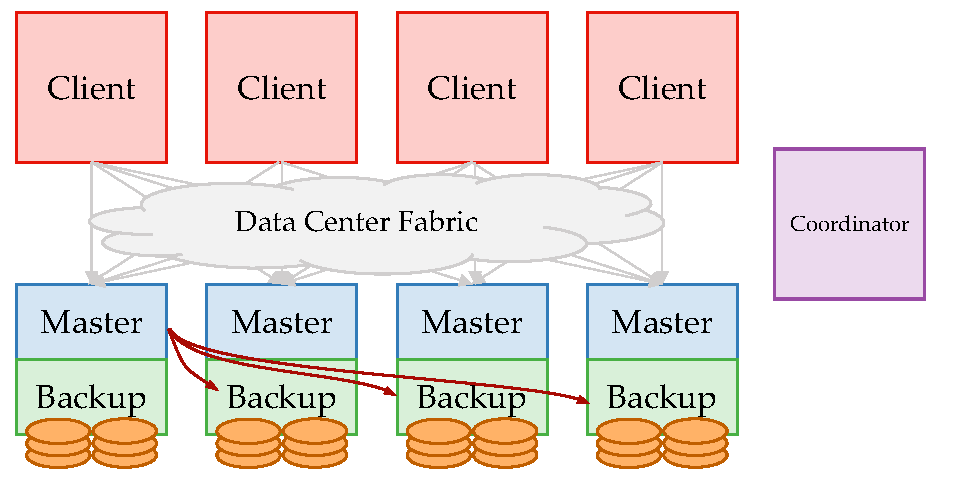
\includegraphics[width=0.8\columnwidth]{figures/ramcloud-cluster.pdf}
\caption{The RAMCloud architecture. Clients issue remote operations
  to RAMCloud storage servers. Each
  server contains a master and a backup. The master component exports the DRAM of
  the server as a large key-value store. The backup accepts updates from other
  masters and records state on disk used for recovering crashed masters. A
  central coordinator manages the server pool and maps data to masters.}
\label{fig:ramcloud-cluster}
\end{figure}


Each server (Figure~\ref{fig:ramcloud-cluster}) operates as a \emph{master},
which manages RAMCloud objects in its DRAM and services client requests, and a
\emph{backup}, which stores redundant copies of objects from other masters on
its local disk.  Each cluster has one quorum-replicated \emph{coordinator} that
manages cluster membership and table-partition-to-master mappings~\cite{ongaro:raft}.

RAMCloud only keeps one copy of each object in memory to avoid replication in
DRAM, which is expensive; it logs redundant copies to (remote) flash.  It provides
high availability with a fast distributed recovery that sprays the objects 
previously hosted on
a failed server across the cluster in
1~to~2~seconds~\cite{ramcloud-recovery}, restoring access to them.
RAMCloud manages
in-memory storage using an approach similar to that of log-structured
filesystems, which allows it to sustain 80-90\% memory utilization
with high performance~\cite{ramcloud-lsm}.

%\noindent
%\textbf{Data Model.}
RAMCloud's design and data model tightly intertwine with load balancing and migration.
Foremost, RAMCloud is a simple variable-length key-value store; its key-space
is divided into unordered tables, and tables can be broken into {\em tablets}
that reside on different servers.  Objects can be accessed by their primary (byte
string) key but ordered secondary indexes can also be constructed on top of
tables~\cite{ramcloud-slik}. Like tables, secondary indexes can be split into
{\em indexlets} to scale them across servers. Indexes contain primary key hashes
rather than records, so tables and their indexes can be scaled independently
and need not be co-located (Figure~\ref{fig:index}). Clients can issue multi-read
and multi-write requests that fetch or modify several objects on one server with
a single request. They can also issue externally consistent and serializable
distributed transactions~\cite{ramcloud-rifl}.

\begin{figure}[t]
\centering
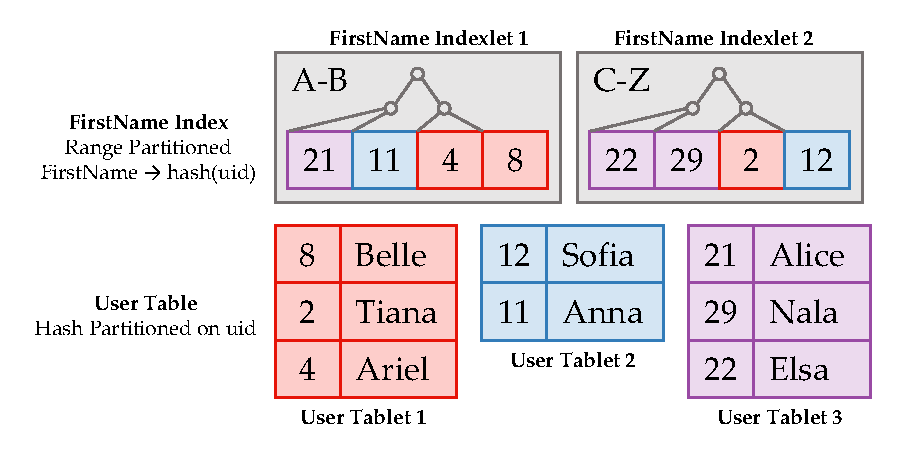
\includegraphics[width=1.0\columnwidth]{figures/ramcloud-index.pdf}
\caption{Index partitioning. Records are stored in unordered tables that can be
  split into tablets on different servers, partitioned on primary key hash.
  Indexes can be range partitioned into indexlets; indexes only contain primary
  key hashes. Range scans require first fetching a list of hashes from an
  indexlet, then multigets for those hashes to the tablet servers to fetch the
  actual records.  A lookup or scan operation is (usually) handled by one
  server, but tables and their indexes can be split and scaled independently.}
\label{fig:index}
\end{figure}


%%K Two things: benefits of locality, inadequacy of existing approaches.
%%K First: locality matters to both client and server performance.
%Two key questions motivate Rocksteady's approach to fast data migration. The
%first question is ``why is migration needed?'' Migration is needed for scaling
%up and down, but it is also needed to manage data locality.  One of the key
%promises of large-scale in-memory systems is predictable low-latency access
%regardless of where values are stored, but, perhaps counterintuitively, careful
%data placement still yields significant gains for both clients and servers.
%Section~\ref{sec:why-balance} below illustrates and shows the gains can be more
%than {\color{red} 7}$\times$.
%
%%K Second: cluster must adapt quickly even though DRAM is growing.
%The second key question is ``what are the key bottlenecks in fast
%reconfiguration?'' Without fast reconfiguration, the cluster cannot react to
%workload changes, even if they are anticipated. Per-server DRAM has continued
%to grow but migration speeds have not. Today's state-of-the-art techniques take
%several hours to move a significant fraction of a server's DRAM~\cite{squall}.
%Section~\ref{sec:bottlenecks} quantifies the bottlenecks in RAMCloud's existing
%migration, which motivates Rocksteady's design that centers around zero-copy
%transmissions and parallelized logical replay.

%DRAM lessens the importance of
%locality within a machine, but careful colocation of correlated keys across the
%cluster can significantly improve total cluster throughput and efficiency.

\subsection{Why Load Balance?}
\label{sec:why-balance}

%K Why not consistent hashing?
All scale-out stores need some way to distribute load across servers.
Most systems today use
some form of consistent
hashing~\cite{chord,dynamo,cassandra}. Consistent hashing is simple,
keeps the key-to-server mapping compact, supports reconfiguration, and
spreads load fairly well even as workloads change. However, its
load spreading is also its drawback; even in-memory stores benefit
significantly from exploiting access locality.

In RAMCloud, for example, co-locating access-correlated keys benefits
multi-get/multi-put operations, transactions, and range queries. Transactions can
benefit significantly if all affected keys can be co-located since
synchronous, remote
coordination for two-phase commit~\cite{ramcloud-rifl,sinfonia} can be avoided.
Multi-operations and range queries benefit in a more subtle but still important
way. If all requested values live together on the same machine, a client can
issue a single remote procedure call (RPC) to a single server to get
the values. If the values are divided among multiple machines, the client must
issue requests to all of the involved machines in parallel. From the client's
perspective, the response latency is similar, but the overall load
induced on the cluster is significantly different.

\begin{figure}[t]
\centering
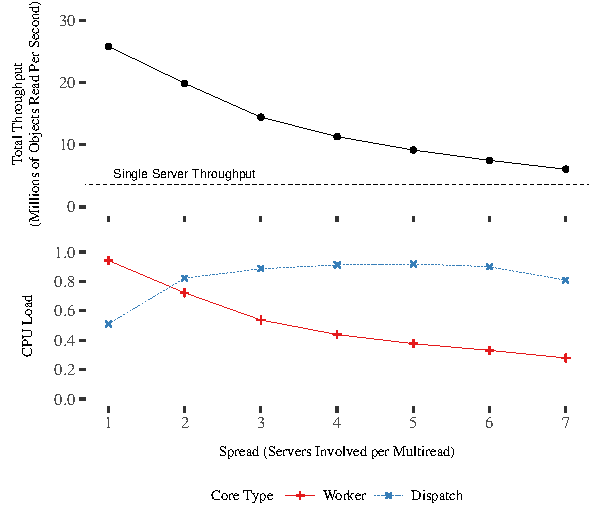
\includegraphics[width=1.0\columnwidth]{graphs/ramcloud-colocation.pdf}
\caption{Throughput and CPU load impact of access locality. When multigets
always fetch data from a single server (Spread~1) throughput is high and
worker cores operate in parallel. When each multiget must fetch keys from
many machines (Spread~7) throughput suffers as each server becomes
bottlenecked on dispatching requests.}
\label{fig:colocation}
\end{figure}


Figure~\ref{fig:colocation} explores this effect. It consists of a
microbenchmark run with seven~servers and 14~client machines. Clients issue back-to-back
multi-get operations evenly across the cluster, each for seven~keys at a time. In
the experiment, clients vary which keys they request in each multi-get to vary
how many servers they must issue parallel requests to, but all servers still
handle the same number of requests as each other.
At Spread~1, all of the keys for a specific multi-get come from one server. At
Spread~2, 6~keys per multi-get come from one server, and the
7\textsuperscript{th} key comes from another server. At Spread~7, each of the
seven~keys in the multi-get is serviced by a different server.

%RAMCloud uses a kernel-bypass networking stack and polls the network device
%(NIC) registers, but each message that is received and dispatched to a worker
%thread induces some load on each server process. When a RAMCloud cluster is
%forced to dispatch 7 requests for 7 objects instead of 1 request for 7
%objects, the total system throughput suffers.
When multi-gets involve two servers rather than one, the cluster-wide throughput
drops 23\% even though no resources have been removed from the cluster. The
bottom half of the figure shows the reason.  Each server has a single {\em dispatch}
core that polls the network device for incoming messages and hands-off requests
to idle {\em worker} cores.  With high locality, the cluster is only limited by
how quickly worker cores can execute requests. When each multi-get results in
requests to two servers, the dispatch core load doubles and saturates, leaving
the workers idle. The dotted line shows the throughput of a single server.
When each multi-get must fetch data from all seven~servers, the entire
cluster's aggregate performance barely outperforms a single machine.

Overall, the experiment shows that, even for small clusters, minimizing tablet
splits and maximizing locality has a significant benefit, in this case, up to
4.3$\times$.  Our findings echo recent trends in scale-out stores that
replicate to minimize multi-get ``fan-out''~\cite{fb-memcache} or give users
explicit control over data placement to exploit locality~\cite{spanner}.

\begin{figure}[t]
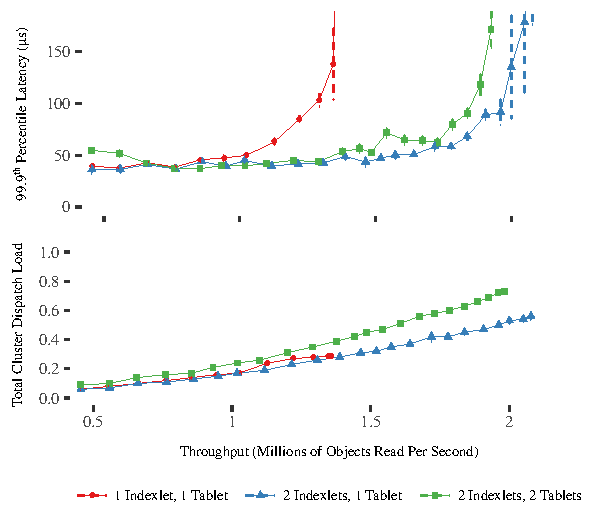
\includegraphics[width=\columnwidth]{graphs/index-motivation}
\caption{Index scaling as a function of read throughput. Points represent
    the median over 5 runs, bars show standard error. Spreading the
    backing table across two servers increases total dispatch load and
    the \nnnth percentile access latency for a given throughput when compared
    to leaving it on a single server.}
\label{fig:index-load}
\end{figure}


Load imbalance has a similar effect on another common case: indexes.
%range-based secondary indexes.  RAMCloud's SLIK~\cite{ramcloud-slik} indexes
%are partitioned ordered B-trees that support range scans on secondary keys.
%The indexes themselves only contain the primary keys of records in their
%leaves.  This allows the indexes themselves to be managed, partitioned, and
%load balanced separately from the tables they index.
Index ranges are especially prone to hotspots, skew shifts, and load increases
that require splits and migration.
%
Figure~\ref{fig:index-load} explores this sensitivity on a cluster with a single
table and secondary index.  The table contains one million 100~B
records, each
with a 30~B primary and a 30~B secondary key. Clients issue short 4-record scans over
the index with the start key chosen from a Zipfian distribution with skew
$\theta$ = 0.5.
%A single run of our experiment issued 10$^{5}$ range scans for a given target
%system throughput.
Figure~\ref{fig:index-load} shows the impact of varying offered client load on
the \nnnth percentile scan latency.

For a target throughput of 1~million objects per second, it is sufficient
(for a \nnnth percentile access latency of 100~\us) and
most efficient (dispatch load is lower) to have the index and table on one server each, but this breaks
down as load increases. At higher loads, \nnnth percentile latency
spikes, and
more servers are needed to bound tail latency. Splitting the index over two
servers improves throughput and restores low access latency.

However, efficiently spreading the load is not straightforward.  Indexes are
range partitioned, so any single scan operation is likely to return hashes using a single
indexlet.  Tables are hash partitioned, so fetching the actual records will
likely result in an RPC to many backing tablets.  As a result, adding tablets for a table
might increase throughput, but it also increases dispatch core load since, cluster-wide,
it requires more RPCs for the same work.

Figure~\ref{fig:index-load} shows that neither minimizing nor maximizing the
number of servers for the indexed table is the best under high load. Leaving the
backing table on one server and spreading the index over two servers increases
throughput at 100~\us \nnnth percentile access latency by 54\% from 1.3 to 2.0
million objects per second. Splitting both the backing table and the index over two
servers gives 6.3\% worse throughput {\em and} increases dispatch load by 26\%.

Overall, reconfiguration is essential to meet SLAs (service level agreements), provide peak throughput,
and minimize load as workloads grow, shrink, and change. Evenly spreading load
is a non-goal as long as SLAs are met; approaches like consistent
hashing can throw away (sometimes large factor) gains from exploiting locality.

\subsection{The Need for (Migration) Speed}

%K DRAM growth fast; network matching, but if migration doesn't we'll be limited.
Data migration speed dictates how fast a cluster can adapt to changing
workloads.  Even if workload shifts are known in advance (like
diurnal patterns), if reconfiguration takes hours, then scaling up and down to
save energy or to do other work becomes impossible.
Recent per-server DRAM capacity growth has been about 33-50\%
per year~\cite{computer-architecture}, making things harder; each server
hosts an ever-increasing amount of
data that may need to move when the cluster is reconfigured.

% Arguments:
%  - DRAM growth doubles every two to three years (Patterson and Hennessey).
%  - Network: 2012 10 Gbps, 2016 40 Gbps: 4x in 4 years, 2x in two years.

A second hardware trend is encouraging; per-host network bandwidth has kept up
with DRAM growth in recent years~\cite{ethernet}, so hardware
itself does not limit fast migration.  For example, an unrealistically large
migration that evacuates half of the data from a 512~GB storage server could
complete in less than a minute at line-rate (5~GB/s or more).

% Squall numbers on Fig 10a: contract from 4 nodes to 3; 2.5 GB of data on the
% source; each cluster member receives (2.5/3 * 1024) = 853 MBs in (220 - 30) =
% 190 seconds. So 4.5 MB/s per target.

Unfortunately, state-of-the-art migration techniques have not kept up
with network improvements. They move data at a few megabytes per second
to minimize the impact on ongoing transactions, and they focus on preserving
transaction latencies on the order of tens of milliseconds~\cite{squall}.
These systems would take more than 16~hours to
migrate 256~GB of data, and small migrations of 10~GB would still take
more than half an hour. Furthermore, modern in-memory systems deliver access
latencies more than 1,000$\times$ lower: in the range of 5~to~50~\us for small
accesses, transactions, or secondary index lookups/scans. If the network
is not a
bottleneck for migration, then what is?

\subsection{Barriers to Fast Migration}
\label{sec:bottlenecks}

RAMCloud has a simple, pre-existing mechanism that allows tables to be split
and migrated between servers.
%It builds on RAMCloud's unique approach to
%distributed recovery~\cite{ramcloud-recovery}.
During normal operation each server stores
all records in an in-memory log. The log is incrementally cleaned; it is
never checkpointed, and a full copy of it always remains in memory.
%a source and target reuse the same mechanisms used for recovery.
To migrate a tablet,
the source iterates over all of the entries in its
in-memory log and copies the values that are being migrated into staging buffers for
transmission to the target. The target receives these buffers and performs a
form of logical replay as it would during recovery. It copies the received
records into its own log, re-replicates them, and it updates its in-memory hash
table, which serves as its primary key index. Only after all of the records
have been transferred is tablet ownership switched from the source to
the target.

\begin{figure}[t]
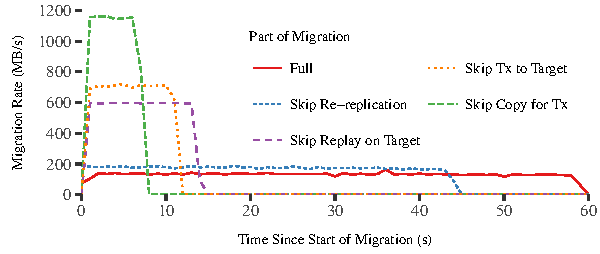
\includegraphics[width=\columnwidth]{graphs/migration-bottlenecks.pdf}
\caption{Bottlenecks when using log replay for migration. Target side
    bottlenecks include logical replay and rereplication.
    Copying records into staging buffers at the source has a
    significant impact on the rate of migration.}
\label{fig:bottlenecks}
\end{figure}


%K possible comparison question: Our old protocol eval was on an unloaded
%K server, it should be slower with load.
%K RAMCloud's old migration design.
%K Also, the old one wasn't two order's' of magnitude slower. 
%K Our NIC line rate < 130*100 MB/s
This basic mechanism is faster than most
approaches,
%and meets SLAs 1,000$\times$ tighter
but it is still orders of
magnitude slower than what hardware can support.  Figure~\ref{fig:bottlenecks}
breaks down its bottlenecks. The
experiment shows the effective migration throughput between a single loaded
source and unloaded target server during the migration of
7~GB of data.  All of the servers are interconnected via 40~Gbps (5~GB/s) links
to a single switch.

The "Full" line shows migration speed when the whole migration
protocol is used. The source scans its log and sends records that need to
be migrated; the target replays the received records into its log and
re-replicates them on backups.
%Once all data has been received the
%source blocks updates for a few hundred microseconds as the last few updates
%are transmitted and ownership is shifted from the source to the target server.
In steady state, migration transfers about 130~MB/s.
% XXX We probably want to say something here about burning cycles waiting on
% re-replication RPCs.

In "Skip Re-Replication" the target skips backing up the
received data in its replicated log. This is unsafe, since the target might accept
updates to the table after it has received all data from the source. If the
target crashes, its recovery log would be missing the data received from the
source, so the received table would be recovered to an inconsistent state.
Even so, migration only reaches 180~MB/s. This shows that the
logical replay used to update the hash table on the target is a key
bottleneck in migration.

"Skip Replay on Target" does the full source-side processing of migration and
transmits the data to the target, but the target skips replay and replication.
This raises migration performance
to 600~MB/s, more than a 3$\times$ increase in migration
rate. Even so, it shows that the source side is also an impediment to fast
migration. The hosts can communicate at 5~GB/s, so the link is still only
about 10\% utilized. Also, at this speed re-replication becomes a
problem; RAMCloud's existing log replication mechanism bottlenecks at around
380~MB/s on our cluster.

Finally, "Skip Tx to Target" performs all source-side processing and skips
transmitting the data to the target, and "Skip Copy for Tx" only identifies
objects that need to be migrated and skips all further work. Overall, copying
the identified objects into staging buffers to be posted to the
transport layer (drop
from 1,150~MB/s to 710~MB/s) has a bigger impact than the actual transmission
itself (drop from 710~MB/s to 600~MB/s).

\subsection{Requirements for a New Design}

These bottlenecks give the design criteria for Rocksteady.

\noindent
\textbf{No Synchronous Re-replication.} Waiting for data to be re-replicated by
the target server wastes CPU cycles on the target waiting for responses from
backups, and it burns memory bandwidth. Rocksteady's approach is inspired by
lineage~\cite{spark}; a target server takes a temporary dependency on the
source's log data to safely eliminate log replication from the migration fast
path (\S\ref{sec:log-dep}).

\noindent
\textbf{Immediate Transfer of Ownership.} RAMCloud's migration takes minutes
or hours during which no load can be shifted away from the source
because the target cannot safely take ownership until all
the data has been re-replicated.  Rocksteady immediately and safely shifts
ownership from the source to the target (\S\ref{sec:new-design}).

% XXX Removed until ZC is added to DPDK tx and evaulated.
%\noindent
%\textbf{Zero-copy Transmission on Source.} Just the cost of packing
%objects into buffers and transmitting them would nearly half migration speed
%(1,150~MB/s to 600~MB/s) even if the target wasn't a bottleneck.

\noindent
\textbf{Parallelism on Both the Target and Source.} Log replay needn't be
single threaded.  A target is likely to be under-loaded, so parallel
replay makes sense. Rocksteady's parallel replay can incorporate log records
at the target at more than 3~GB/s (\S\ref{sec:eval-replay}). Similarly,
source-side migration operations should be pipelined and parallel. Parallelism
on both ends requires care to avoid contention.

\noindent
\textbf{Load-Adaptive Replay.} Rocksteady's migration manager minimizes impact
on normal request processing with fine-grained low-priority
tasks~\cite{morsel-driven-parallelism,sparrow}. Rocksteady also incorporates
into RAMCloud's transport layer to minimize jitter caused by background
migration transfers (\S\ref{sec:qos}).
